\documentclass[a4paper,12pt]{article}
\usepackage[utf8]{inputenc}

\usepackage[utf8]{inputenc}
\usepackage[T2A]{fontenc}
\usepackage[english,russian]{babel}
\usepackage{amsthm}
\usepackage{amsmath}
\usepackage{amssymb}
\usepackage{tikz}
\usepackage{textcomp}
\usepackage{marvosym}
\usepackage{ esint }
\usepackage{mathtext}
\usepackage{siunitx} % Required for alignment
\usepackage{subfigure}
\usepackage{multirow}
\usepackage{rotating}
\usepackage{afterpage}
\usepackage[arrowdel]{physics}
\usepackage{booktabs}
\setlength{\topmargin}{-0.5in}
\setlength{\textheight}{9.1in}
\setlength{\oddsidemargin}{-0.4in}
\setlength{\evensidemargin}{-0.4in}
\setlength{\textwidth}{7in}
\setlength{\parindent}{0ex}
\setlength{\parskip}{1ex}
\newcommand{\ndiv}{\hspace{-4pt}\not|\hspace{2pt}}
\usepackage{graphicx}
\usepackage{float}
\usepackage{wrapfig}
\usepackage{pgfplots}
\usepackage{caption}
\pgfplotsset{compat=1.16}
\graphicspath{ {./images/} }
\usepackage{graphicx}
\RequirePackage{caption}
\DeclareCaptionLabelSeparator{defffis}{ — }
\captionsetup{justification=centering,labelsep=defffis}
\usepackage{caption} \captionsetup[table]{labelsep=endash,justification=justified,singlelinecheck=false,font=normalsize}
\usepackage{amsfonts,mathtools}
\title{Лабораторная работа № 4.3.6\\Саморепродукция}
\author{Пазов Тенгиз, Симухин Егор}
\date{Март 2025}

\begin{document}
\maketitle
\begin{figure}[h!]
\centering

\includegraphics[scale=0.25]{MIPT.jpg}
\end{figure}
\newpage
\section*{Введение}
\textbf{Цель работы:} Изучение явления саморепродукции и применение его к измерению параметров периодических структур.

\textbf{В работе используются:} лазер, кассета с сетками, мира, короткофокусная линза с микрометрическим винтом, экран, линейка.

\section{Теоретическая часть}
При дифракции на предмете с периодической структурой наблюдается интересное явление: на некотором расстоянии от предмета вдоль направления распространения волны появляется изображение, которое потом периодически повторяется — репродуцируется

Этот эффект имеет простое физическое объяснение. Если на
пути распространения плоской волны в плоскости z = 0 расположить транспарант (например, изображение предмета на фотоплёнке или стеклянной пластинке) с функцией пропускания, отличной от константы, то на выходе из него в плоскости z = 0+
волна уже перестанет быть плоской. Если при этом функция пропускания транспаранта — периодическая функция координат, периодической функцией будет и комплексная амплитуда волны на
выходе из транспаранта, т. е. в плоскости z = 0+. Периодическому распределению комплексной амплитуды в плоскости z = 0+
будет соответствовать дискретный набор плоских волн с кратными пространственными частотами. При этом оказывается, что существуют плоскости (при z > 0), где все плоские волны имеют
те же самые фазовые соотношения, что и в плоскости z = 0+.

Легко видеть, что в плоскости наблюдения $z_0 = \frac{2d_2}{\lambda}$ разность фазовых набегов оказывается кратной $2\pi$ для любых гармоник, 5 входящих
в состав суперпозиции, т. е. совпадают фазовые соотношения между
колебаниями, которые создаются всеми плоскими волнами, входящими в состав суперпозиции (4) в предметной плоскости z = 0+ и в плоскости изображения $z_1 = \frac{2d_2}{\lambda}$. Поэтому в результате интерференции этих волн мы получаем изображение, тождественное исходному периодическому объекту. Описанное явление называется эффектом саморепродукции. Световая волна сама (без каких-либо линз или зеркал) создает изображение исходного объекта. Все сказанное справедливо и для любого расстояния $z_N$, кратного $z_1$:
\begin{equation}
z_N = \frac{2 \cdot d^2}{\lambda} \cdot N
\end{equation}

На опыте, вследствие ограниченности поперечного сечения светового пучка лазера, наблюдаются только несколько репродуцированных изображений решетки. Поясним этот эффект с помощью рис. 1. 

На нем изображены только три продифрагировавших луча соответственно нулевого (n = 0) и $\pm$ первого порядка (n = $\pm 1$). Там, где эти лучи перекрываются, образуется интерференционная картина с периодом, как раз равным периоду решетки d.
Спроектировав картину с помощью линзы на экран, мы увидим изображения синусоидальной решетки с плавным переходом от максимумов к минимумам. Для того чтобы наблюдать более тонкие детали, необходимо, чтобы в плоскости наблюдения перекрывались лучи более высоких дифракционных порядков. На краях, где перекрываютcя только два луча (n = 0 и n = +1 или n = 0 и n = -1), также образуется интерференционная картина с периодом d, но менее контрастная.
\begin{figure}[H]
\centering
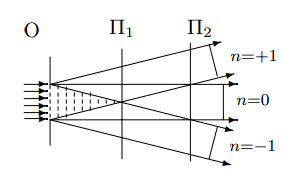
\includegraphics[scale=1]{scheme1.png}
\caption{Принципиальная схема дифракции на сетке. Между сеткой 0 и плоскостью $\text{П}_1$ наблюдаются репродуцированные изображения сетки}
\end{figure}
\section{Экспериментальная установка}
Хорошим приближением к плоской волне в нашем эксперименте является излучение лазера. Луч лазера падает перпендикулярно на периодический объект О, установленный в плоскости $P_0$ (рис. 2).

За плоскостью $P_0$ (в плоскостях $P_1$–$P_N$) периодически по z возникают изображения объекта, которые с помощью линзы Л можно поочерёдно проецировать на экран, установленный в плоскости Э. Если убрать линзу, то на экране наблюдается картина дифракции луча лазера на периодическом объекте.

\begin{figure}[H]
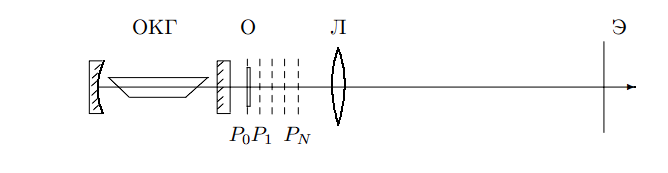
\includegraphics[scale=1]{scheme2.png}
\caption{Схема установки: ОКГ - гелий-неоновый лазер, 0 - двумерная решётка, $P_N$ - плоскости, где наблюдаются репродуцированные изображения, Л - короткофокусная линза, Э - экран для наблюдения изображения объекта}
\end{figure}

Экран устанавливается достаточно далеко от объекта, так что продифрагировавшие лучи, соответствующие различным порядкам дифракции ($\sin \varphi_n = \frac{n\lambda}{d}$), разделяются. 

Измерив расстояние между дифракционными максимумами и расстояние от объекта до экрана, мы определим $\sin \varphi_n$ и d.

В нашей работе в качестве периодических объектов применяется мира — набор различным образом ориентированных одномерных решеток разного периода (рис. 4), а
также двумерная решетка-сетка. Сетку можно рассматривать как две взаимно перпендикулярные решетки. Узкий пучок монохроматического света, пройдя через первую решетку с вертикальными штрихами, должен дать совокупность максимумов, расположенных вдоль горизонтальной линии.

Световой пучок, соответствующий каждому максимуму, проходя через вторую решетку, распадается на новую совокупность пучков, дающих максимумы вдоль вертикальной линии. В результате главные максимумы возникают тогда, когда одновременно выполняются условия
\begin{equation}
d \sin \varphi_x = n_x \lambda, d \sin \varphi_y = n_y \lambda 
\end{equation}
где $n_x$ и $n_y$ — два целых числа, характеризующих порядки дифракционных максимумов, $\varphi_x$ и $\varphi_y$ — направления на главные дифракционные максимумы в горизонтальной и вертикальной плоскостях соответственно (рис. 3). Максимумы показаны кружками, размеры которых характеризуют интенсивность.
\begin{figure}[H]
	\centering
	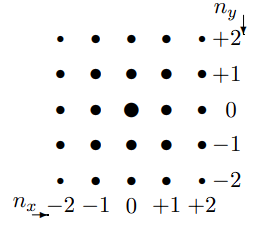
\includegraphics[scale=1]{scheme3.png}
	\caption{Спектр решётки}
\end{figure}
\section{Ход работы}
\subsection*{Определение периода решёток по их пространственному спектру}
Для начала установим вблизи лазера кассету с двумерными решётками(сетками). Затем для каждой из сеток(в нашем случае их было $5$), измерим расстояние $x$ между двумя соседними дифракционными максимумами на экране. Также измерим расстояние $L$ от кассеты до экрана. Оно получилось равным $1337 \pm 1$ мм. Длина волны зелёного лазера $\lambda = 532$ нм. Зная $x$ и $L$, вычислим период решётки по формуле (2), считая $\sin \varphi \approx \varphi \approx \frac{x}{L}$.$X$ - расстояние между максимумами $\sigma_X = 1$ мм, m - количество промежутков между этими максимумами.
\begin{table}[H]
	\centering
	\begin{tabular}{|c|c|c|c|c|c|}
	\hline
	№ сетки & X, мм & m & x, мм & $d_\text{сп}$, мкм & $\sigma_{d_\text{сп}}$, мкм\\ \hline
	1 & 144 & 4 & 36 & 19,7 & 0,7\\ \hline
	2 & 145 & 6 & 24,1 & 29,5 & 1,3\\ \hline
	3 & 156 & 13 & 12 & 59,3 & 5,3\\ \hline
	4 & 96 & 16 & 6 & 118,5 & 11,2\\ \hline
	5 & 150 & 33 & 4,54 & 156,7 & 13,1\\ \hline
	\end{tabular}
\end{table}
\subsection*{Определение периода решёток по изображению, увеличенному с помощью линзы}
Теперь установим короткофокусную линзу на небольшом расстоянии от лазера, между ней и лазером установим кассету с сетками, настроим систему так, чтобы было видно резкое изобрадение проволочки(т.е. непериодического объекта). Определим размеры D клеток на экране для всех сеток, для которых это возможно. Также измерим расстояния от линзы до сетки (a) и до экрана (b). $a = 50 \pm 1$ мм, $b = 1300 \pm 1$ мм. По этим измерениям по формуле $ d_\text{л} = \frac{Da}{b}$ рассчитаем периоды сеток.

\begin{table}[H]
	\centering
	\begin{tabular}{|c|c|c|c|c|}
	\hline
	№ сетки & D, мм & $\sigma_D$, мм & $d_\text{л}$, мкм & $\sigma_{d_\text{л}}$, мкм \\ \hline
	2 & 0,9 & 0,1 & 34,6 & 2.7 \\ \hline
	3 & 1,8 & 0,1 & 69,2 & 5.3 \\ \hline
	4 & 3 & 0,1 & 115,4 & 8.9 \\ \hline
	5 & 4 & 0,1 & 153,8 & 11.8 \\ \hline
	\end{tabular}
\end{table}

\subsection*{Исследование эффекта саморепродукции с помощью сеток}
Далее получим на экране геометрическое изображение сетки. Затем, перемещая линзу с помощью микровинта, определим по нониусной шкале координаты $z_N$ плоскостей саморепродукции, соотвтетствующих чёткому изображению сетки на экране. По полученным данным построим графики зависимости $z_N = f(N)$, при помощи которых по наклону прямых рассчитаем периоды сеток $d_\text{реп}$ по формуле (1).
\begin{figure}[H]
\centering
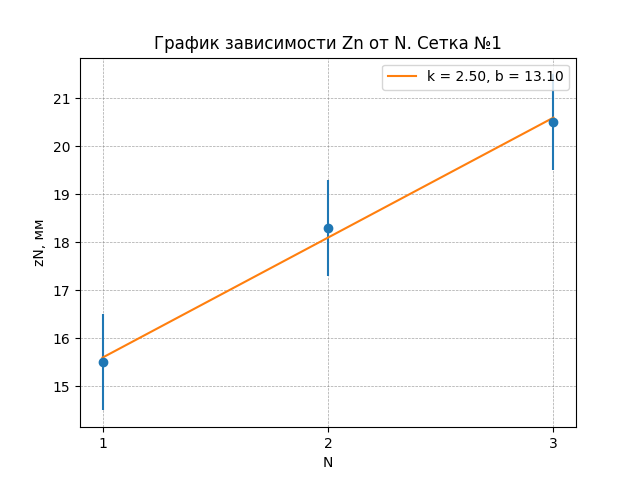
\includegraphics[scale=0.65]{1.png}

\end{figure}

\begin{figure}[H]
\centering
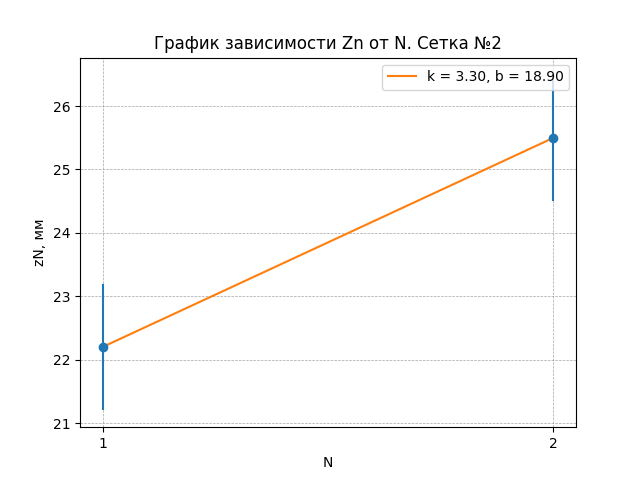
\includegraphics[scale=0.65]{2.png}

\end{figure}

\begin{figure}[H]
\centering
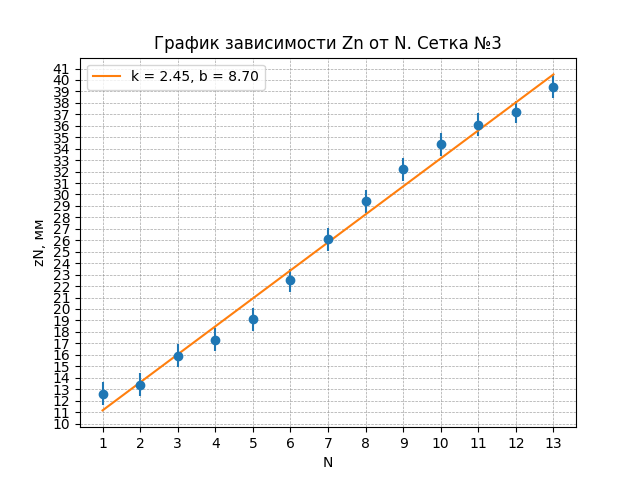
\includegraphics[scale=1]{3.png}

\end{figure}

\begin{table}[H]
\centering
\begin{tabular}{|c|c|c|}
\hline
 № сетки & $d_\text{реп}$, мм & $\sigma_{d_\text{реп}}$, мкм \\ \hline
 1 & 25,8 & 0,1 \\ \hline
 2 & 29,6 & nan \\ \hline
 3 & 25,5 & 0,1 \\ \hline
 4 & 37,9 & 0,4 \\ \hline
 5 & 52,8 & 0,5 \\ \hline
\end{tabular}
\end{table}
\begin{table}[H]
\centering
	\begin{tabular}{|c|c|c|c|}
	\hline
	№ сетки & $d_\text{сп}$, мкм & $d_\text{л}$, мкм & $d_\text{реп}$, мкм\\ \hline
	1 & 19,7 & -- & 25,8\\ \hline
	2 & 29,5 & 34,6 & 29,6\\ \hline
	3 & 59,3 & 69,2 &  25,5\\ \hline
	4 & 118,5 & 115,4 & 37,9 \\ \hline
	5 & 156,7 & 153,8 & 52,8a\\ \hline
	
	\end{tabular}
\end{table}
\subsection*{Исследование решёток миры}
Теперь установим миру на место кассеты. Вычисления будут произведены для элементов миры под номером 20 и 25. 

Измерим период миры теми же способами, что использовались до этого. Расстояние от линзы до миры $a = 50 \pm 1 $мм. Расстояние от линзы до экрана $b = 1260 \pm 1$ мм. Соответственно расстояние от миры до экрана равно $L = 1347 \pm 1$ мм.

Определим по нониусной шкале координату плоскости, соответствующей изображению миры на экране по законам геометрической оптики(нет рассеяния, чёткая картина). $z_{25} = -10,4 \pm 0,1$ мм, $z_{20} = -14,0 \pm 0,1$ мм. На этих координатах, вычислив значение $D$, получим значение $d_\text{л}$.

Также построим график зависимости $z_N = f(N)$, где $z_N$ - координаты на нониусной шкале плоскостей саморепродукции.

И в конце, убрав линзу и вычислив расстояние между максимумами, определим $d_\text{сп}$.

\begin{figure}[H]
\centering
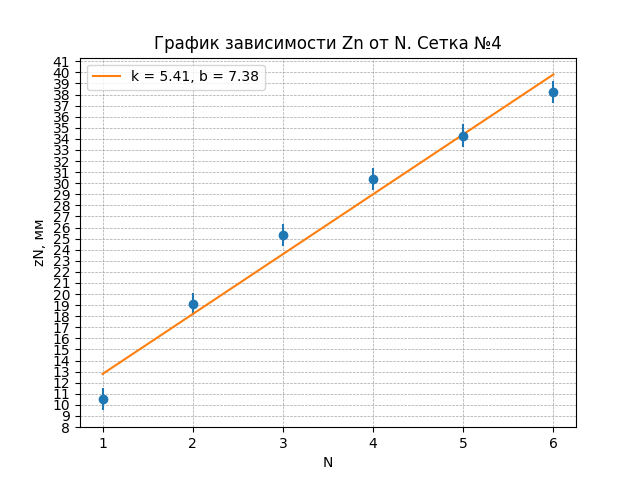
\includegraphics[scale=0.65]{4.png}
\end{figure}


\begin{figure}[H]
\centering
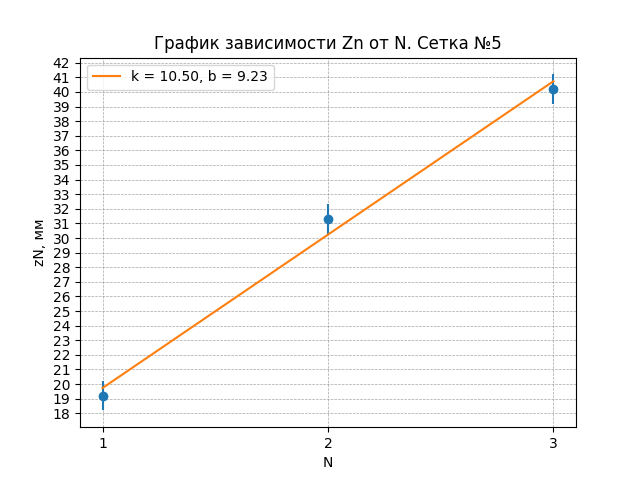
\includegraphics[scale=0.65]{5.png}
\end{figure}

Полученные результаты приведены в таблице.
\begin{table}[H]
\begin{tabular}{|c|c|c|c|c|c|c|}
\hline
№ элемента миры & $d_\text{сп}$, мкм & $\sigma_{d_\text{сп}}$, мкм & $d_\text{л}$, мкм & $\sigma_{d_\text{л}}$, мкм & $d_\text{реп}$, мкм & $\sigma_{d_\text{реп}}$, мкм \\ \hline
25 & 38,76 & 0,18 & 40,1 & 0,2 & 29,9 & 0,8 \\ \hline
20 & 51,7 & 0,2 & 53,5 & 0,3 & 37,2 & 0,4 \\ \hline
\end{tabular}
\end{table}
\begin{figure}[H]
\centering
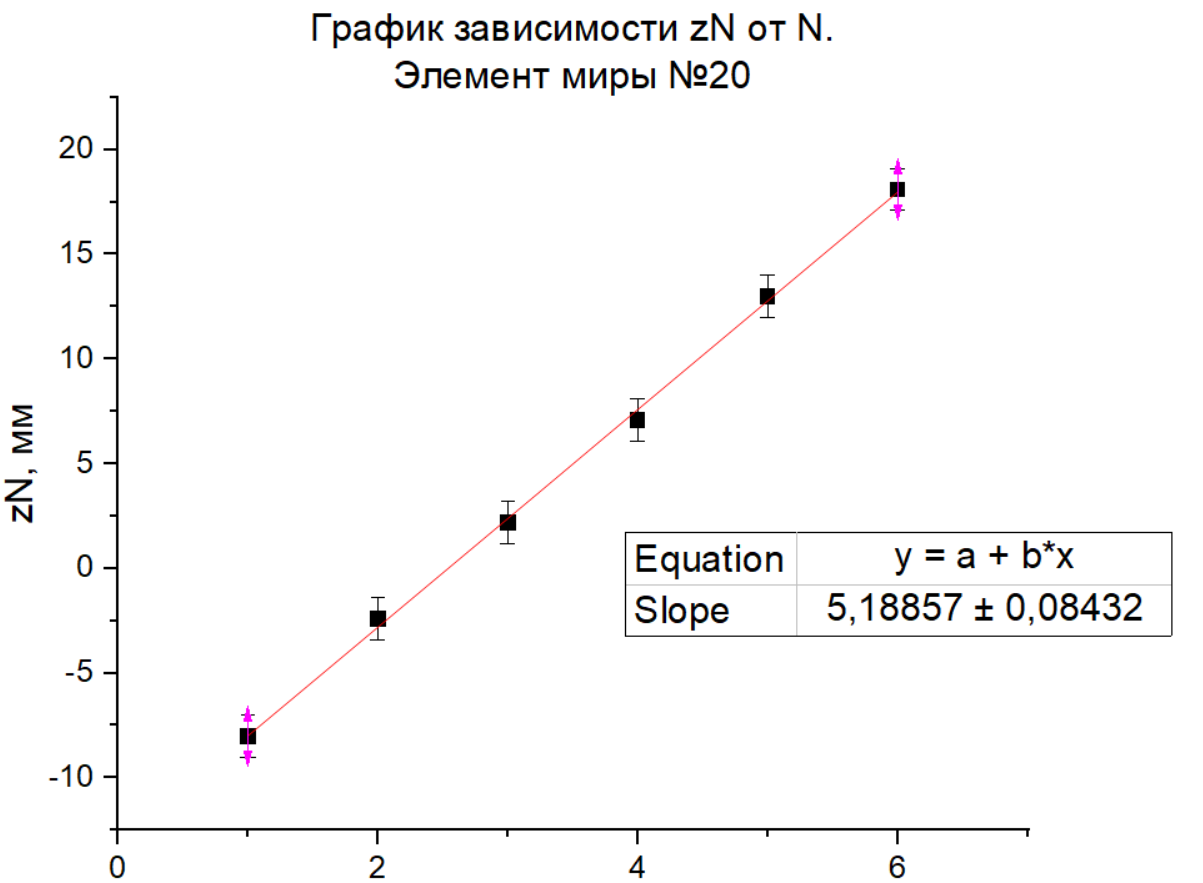
\includegraphics[scale=0.4]{6.png}
\end{figure}
\begin{figure}[H]
\centering
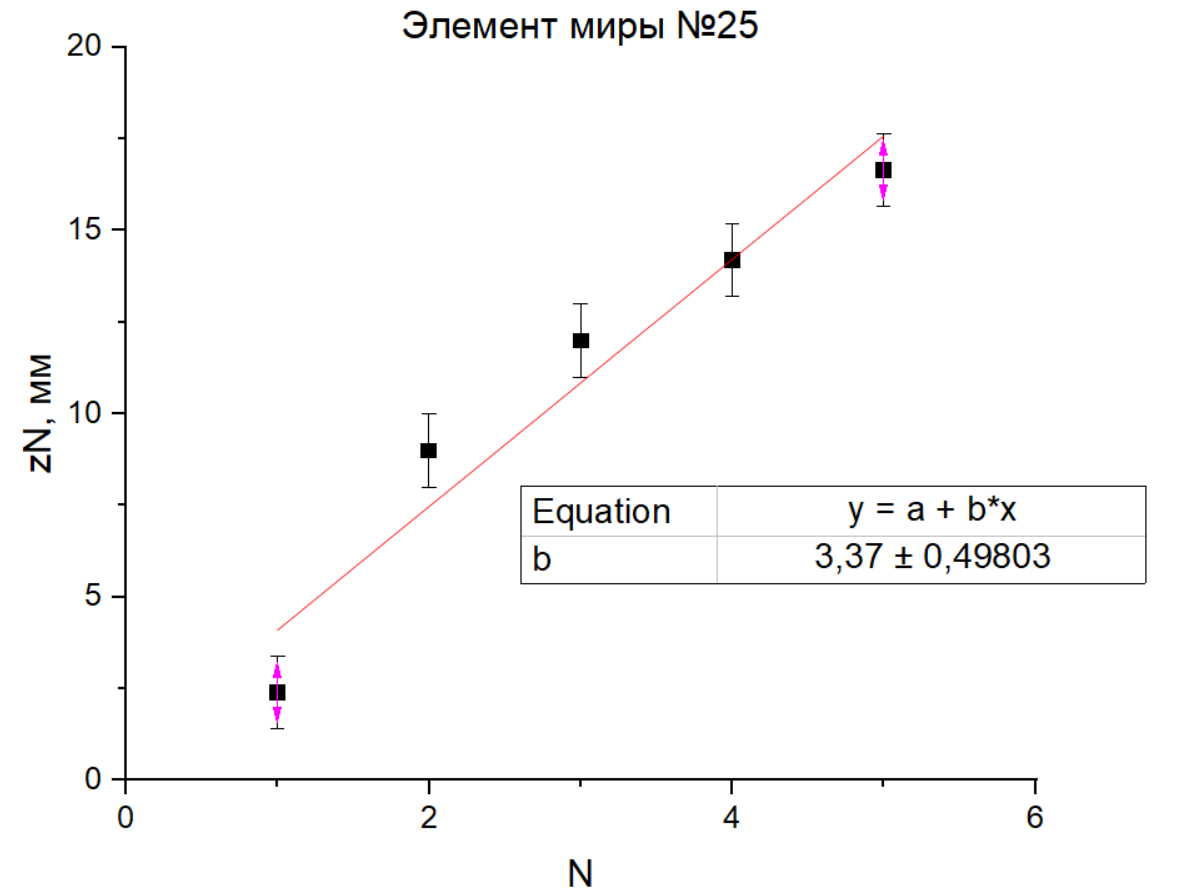
\includegraphics[scale=0.4]{7.png}
\end{figure}
\section{Вывод}
В ходе данной работы было изучено явления саморепродукции. Также данное явление было использовано для измерения параметров периодических структур. Так, в процессе работы был измерен период решётки тремя различными способами, одним из которых и было применение саморепродукции. В результате этих измерений было получено, что значения, измеренные первыми двумя способами, в отличие от 3ого способа находятся достаточно близко друг к другу(результаты были приведены в таблице), что говорит о работе данного метода по измерению параметров периодических структур. Это также было продемонстрировано на работе с решётками миры. 
\end{document}